\documentclass{article}\usepackage[]{graphicx}\usepackage[]{xcolor}
% maxwidth is the original width if it is less than linewidth
% otherwise use linewidth (to make sure the graphics do not exceed the margin)
\makeatletter
\def\maxwidth{ %
  \ifdim\Gin@nat@width>\linewidth
    \linewidth
  \else
    \Gin@nat@width
  \fi
}
\makeatother

\definecolor{fgcolor}{rgb}{0.345, 0.345, 0.345}
\newcommand{\hlnum}[1]{\textcolor[rgb]{0.686,0.059,0.569}{#1}}%
\newcommand{\hlstr}[1]{\textcolor[rgb]{0.192,0.494,0.8}{#1}}%
\newcommand{\hlcom}[1]{\textcolor[rgb]{0.678,0.584,0.686}{\textit{#1}}}%
\newcommand{\hlopt}[1]{\textcolor[rgb]{0,0,0}{#1}}%
\newcommand{\hlstd}[1]{\textcolor[rgb]{0.345,0.345,0.345}{#1}}%
\newcommand{\hlkwa}[1]{\textcolor[rgb]{0.161,0.373,0.58}{\textbf{#1}}}%
\newcommand{\hlkwb}[1]{\textcolor[rgb]{0.69,0.353,0.396}{#1}}%
\newcommand{\hlkwc}[1]{\textcolor[rgb]{0.333,0.667,0.333}{#1}}%
\newcommand{\hlkwd}[1]{\textcolor[rgb]{0.737,0.353,0.396}{\textbf{#1}}}%
\let\hlipl\hlkwb

\usepackage{framed}
\makeatletter
\newenvironment{kframe}{%
 \def\at@end@of@kframe{}%
 \ifinner\ifhmode%
  \def\at@end@of@kframe{\end{minipage}}%
  \begin{minipage}{\columnwidth}%
 \fi\fi%
 \def\FrameCommand##1{\hskip\@totalleftmargin \hskip-\fboxsep
 \colorbox{shadecolor}{##1}\hskip-\fboxsep
     % There is no \\@totalrightmargin, so:
     \hskip-\linewidth \hskip-\@totalleftmargin \hskip\columnwidth}%
 \MakeFramed {\advance\hsize-\width
   \@totalleftmargin\z@ \linewidth\hsize
   \@setminipage}}%
 {\par\unskip\endMakeFramed%
 \at@end@of@kframe}
\makeatother

\definecolor{shadecolor}{rgb}{.97, .97, .97}
\definecolor{messagecolor}{rgb}{0, 0, 0}
\definecolor{warningcolor}{rgb}{1, 0, 1}
\definecolor{errorcolor}{rgb}{1, 0, 0}
\newenvironment{knitrout}{}{} % an empty environment to be redefined in TeX

\usepackage{alltt}
\usepackage[sc]{mathpazo}
\renewcommand{\sfdefault}{lmss}
\renewcommand{\ttdefault}{lmtt}
\usepackage[T1]{fontenc}
\usepackage{geometry}
\geometry{verbose,tmargin=2.5cm,bmargin=2.5cm,lmargin=2.5cm,rmargin=2.5cm}
\setcounter{secnumdepth}{2}
\setcounter{tocdepth}{2}
\usepackage[unicode=true,pdfusetitle,
 bookmarks=true,bookmarksnumbered=true,bookmarksopen=true,bookmarksopenlevel=2,
 breaklinks=false,pdfborder={0 0 1},backref=false,colorlinks=false]
 {hyperref}
\hypersetup{
 pdfstartview={XYZ null null 1}}

\makeatletter
%%%%%%%%%%%%%%%%%%%%%%%%%%%%%% User specified LaTeX commands.
\renewcommand{\textfraction}{0.05}
\renewcommand{\topfraction}{0.8}
\renewcommand{\bottomfraction}{0.8}
\renewcommand{\floatpagefraction}{0.75}

\makeatother
\IfFileExists{upquote.sty}{\usepackage{upquote}}{}
\begin{document}



\title{\title{\title{\title{\title{\title{\title{\title{\title{\title{}}}}}}}}}}



\maketitle
The results below are generated from an R script.

\begin{knitrout}
\definecolor{shadecolor}{rgb}{0.969, 0.969, 0.969}\color{fgcolor}\begin{kframe}
\begin{alltt}
\hlcom{# Liberías necesarias para resolver el ejercicio}
\hlkwd{library}\hlstd{(ISLR2)}
\hlkwd{library}\hlstd{(ggplot2)}
\hlkwd{library}\hlstd{(randomForest)}
\hlkwd{library}\hlstd{(ROCR)}
\hlkwd{library}\hlstd{(}\hlstr{"DALEX"}\hlstd{)}

\hlcom{# Variable respuesta a factor}
\hlstd{car}\hlkwb{=}\hlstd{Caravan}
\hlstd{car}\hlopt{$}\hlstd{Purchase}\hlkwb{=}\hlkwd{as.factor}\hlstd{(car}\hlopt{$}\hlstd{Purchase)}
\hlcom{# Dividimos la muestra en train, test}
\hlcom{# Parciticionamos los datos}
\hlkwd{set.seed}\hlstd{(}\hlnum{2138}\hlstd{)}
\hlstd{n}\hlkwb{=}\hlkwd{dim}\hlstd{(car)[}\hlnum{1}\hlstd{]}
\hlstd{indices}\hlkwb{=}\hlkwd{seq}\hlstd{(}\hlnum{1}\hlopt{:}\hlstd{n)}
\hlstd{indices.train}\hlkwb{=}\hlkwd{sample}\hlstd{(indices,}\hlkwc{size}\hlstd{=n}\hlopt{*}\hlnum{.8}\hlstd{,}\hlkwc{replace}\hlstd{=}\hlnum{FALSE}\hlstd{)}
\hlstd{indices.test}\hlkwb{=}\hlkwd{sample}\hlstd{(indices[}\hlopt{-}\hlstd{indices.train],}\hlkwc{size}\hlstd{=n}\hlopt{*}\hlnum{.1}\hlstd{,}\hlkwc{replace}\hlstd{=}\hlnum{FALSE}\hlstd{)}
\hlstd{indices.valid}\hlkwb{=}\hlstd{indices[}\hlopt{-}\hlkwd{c}\hlstd{(indices.train,indices.test)]}

\hlstd{car.train}\hlkwb{=}\hlstd{car[indices.train,]}
\hlstd{car.test}\hlkwb{=}\hlstd{car[indices.test,]}
\hlstd{car.valid}\hlkwb{=}\hlstd{car[indices.valid,]}

\hlcom{# EDA}
\hlkwd{str}\hlstd{(Caravan)}
\end{alltt}
\begin{verbatim}
## 'data.frame':	5822 obs. of  86 variables:
##  $ MOSTYPE : num  33 37 37 9 40 23 39 33 33 11 ...
##  $ MAANTHUI: num  1 1 1 1 1 1 2 1 1 2 ...
##  $ MGEMOMV : num  3 2 2 3 4 2 3 2 2 3 ...
##  $ MGEMLEEF: num  2 2 2 3 2 1 2 3 4 3 ...
##  $ MOSHOOFD: num  8 8 8 3 10 5 9 8 8 3 ...
##  $ MGODRK  : num  0 1 0 2 1 0 2 0 0 3 ...
##  $ MGODPR  : num  5 4 4 3 4 5 2 7 1 5 ...
##  $ MGODOV  : num  1 1 2 2 1 0 0 0 3 0 ...
##  $ MGODGE  : num  3 4 4 4 4 5 5 2 6 2 ...
##  $ MRELGE  : num  7 6 3 5 7 0 7 7 6 7 ...
##  $ MRELSA  : num  0 2 2 2 1 6 2 2 0 0 ...
##  $ MRELOV  : num  2 2 4 2 2 3 0 0 3 2 ...
##  $ MFALLEEN: num  1 0 4 2 2 3 0 0 3 2 ...
##  $ MFGEKIND: num  2 4 4 3 4 5 3 5 3 2 ...
##  $ MFWEKIND: num  6 5 2 4 4 2 6 4 3 6 ...
##  $ MOPLHOOG: num  1 0 0 3 5 0 0 0 0 0 ...
##  $ MOPLMIDD: num  2 5 5 4 4 5 4 3 1 4 ...
##  $ MOPLLAAG: num  7 4 4 2 0 4 5 6 8 5 ...
##  $ MBERHOOG: num  1 0 0 4 0 2 0 2 1 2 ...
##  $ MBERZELF: num  0 0 0 0 5 0 0 0 1 0 ...
##  $ MBERBOER: num  1 0 0 0 4 0 0 0 0 0 ...
##  $ MBERMIDD: num  2 5 7 3 0 4 4 2 1 3 ...
##  $ MBERARBG: num  5 0 0 1 0 2 1 5 8 3 ...
##  $ MBERARBO: num  2 4 2 2 0 2 5 2 1 3 ...
##  $ MSKA    : num  1 0 0 3 9 2 0 2 1 1 ...
##  $ MSKB1   : num  1 2 5 2 0 2 1 1 1 2 ...
##  $ MSKB2   : num  2 3 0 1 0 2 4 2 0 1 ...
##  $ MSKC    : num  6 5 4 4 0 4 5 5 8 4 ...
##  $ MSKD    : num  1 0 0 0 0 2 0 2 1 2 ...
##  $ MHHUUR  : num  1 2 7 5 4 9 6 0 9 0 ...
##  $ MHKOOP  : num  8 7 2 4 5 0 3 9 0 9 ...
##  $ MAUT1   : num  8 7 7 9 6 5 8 4 5 6 ...
##  $ MAUT2   : num  0 1 0 0 2 3 0 4 2 1 ...
##  $ MAUT0   : num  1 2 2 0 1 3 1 2 3 2 ...
##  $ MZFONDS : num  8 6 9 7 5 9 9 6 7 6 ...
##  $ MZPART  : num  1 3 0 2 4 0 0 3 2 3 ...
##  $ MINKM30 : num  0 2 4 1 0 5 4 2 7 2 ...
##  $ MINK3045: num  4 0 5 5 0 2 3 5 2 3 ...
##  $ MINK4575: num  5 5 0 3 9 3 3 3 1 3 ...
##  $ MINK7512: num  0 2 0 0 0 0 0 0 0 1 ...
##  $ MINK123M: num  0 0 0 0 0 0 0 0 0 0 ...
##  $ MINKGEM : num  4 5 3 4 6 3 3 3 2 4 ...
##  $ MKOOPKLA: num  3 4 4 4 3 3 5 3 3 7 ...
##  $ PWAPART : num  0 2 2 0 0 0 0 0 0 2 ...
##  $ PWABEDR : num  0 0 0 0 0 0 0 0 0 0 ...
##  $ PWALAND : num  0 0 0 0 0 0 0 0 0 0 ...
##  $ PPERSAUT: num  6 0 6 6 0 6 6 0 5 0 ...
##  $ PBESAUT : num  0 0 0 0 0 0 0 0 0 0 ...
##  $ PMOTSCO : num  0 0 0 0 0 0 0 0 0 0 ...
##  $ PVRAAUT : num  0 0 0 0 0 0 0 0 0 0 ...
##  $ PAANHANG: num  0 0 0 0 0 0 0 0 0 0 ...
##  $ PTRACTOR: num  0 0 0 0 0 0 0 0 0 0 ...
##  $ PWERKT  : num  0 0 0 0 0 0 0 0 0 0 ...
##  $ PBROM   : num  0 0 0 0 0 0 0 3 0 0 ...
##  $ PLEVEN  : num  0 0 0 0 0 0 0 0 0 0 ...
##  $ PPERSONG: num  0 0 0 0 0 0 0 0 0 0 ...
##  $ PGEZONG : num  0 0 0 0 0 0 0 0 0 0 ...
##  $ PWAOREG : num  0 0 0 0 0 0 0 0 0 0 ...
##  $ PBRAND  : num  5 2 2 2 6 0 0 0 0 3 ...
##  $ PZEILPL : num  0 0 0 0 0 0 0 0 0 0 ...
##  $ PPLEZIER: num  0 0 0 0 0 0 0 0 0 0 ...
##  $ PFIETS  : num  0 0 0 0 0 0 0 0 0 0 ...
##  $ PINBOED : num  0 0 0 0 0 0 0 0 0 0 ...
##  $ PBYSTAND: num  0 0 0 0 0 0 0 0 0 0 ...
##  $ AWAPART : num  0 2 1 0 0 0 0 0 0 1 ...
##  $ AWABEDR : num  0 0 0 0 0 0 0 0 0 0 ...
##  $ AWALAND : num  0 0 0 0 0 0 0 0 0 0 ...
##  $ APERSAUT: num  1 0 1 1 0 1 1 0 1 0 ...
##  $ ABESAUT : num  0 0 0 0 0 0 0 0 0 0 ...
##  $ AMOTSCO : num  0 0 0 0 0 0 0 0 0 0 ...
##  $ AVRAAUT : num  0 0 0 0 0 0 0 0 0 0 ...
##  $ AAANHANG: num  0 0 0 0 0 0 0 0 0 0 ...
##  $ ATRACTOR: num  0 0 0 0 0 0 0 0 0 0 ...
##  $ AWERKT  : num  0 0 0 0 0 0 0 0 0 0 ...
##  $ ABROM   : num  0 0 0 0 0 0 0 1 0 0 ...
##  $ ALEVEN  : num  0 0 0 0 0 0 0 0 0 0 ...
##  $ APERSONG: num  0 0 0 0 0 0 0 0 0 0 ...
##  $ AGEZONG : num  0 0 0 0 0 0 0 0 0 0 ...
##  $ AWAOREG : num  0 0 0 0 0 0 0 0 0 0 ...
##  $ ABRAND  : num  1 1 1 1 1 0 0 0 0 1 ...
##  $ AZEILPL : num  0 0 0 0 0 0 0 0 0 0 ...
##  $ APLEZIER: num  0 0 0 0 0 0 0 0 0 0 ...
##  $ AFIETS  : num  0 0 0 0 0 0 0 0 0 0 ...
##  $ AINBOED : num  0 0 0 0 0 0 0 0 0 0 ...
##  $ ABYSTAND: num  0 0 0 0 0 0 0 0 0 0 ...
##  $ Purchase: Factor w/ 2 levels "No","Yes": 1 1 1 1 1 1 1 1 1 1 ...
\end{verbatim}
\begin{alltt}
\hlkwd{summary}\hlstd{(car.train)}
\end{alltt}
\begin{verbatim}
##     MOSTYPE         MAANTHUI         MGEMOMV         MGEMLEEF        MOSHOOFD     
##  Min.   : 1.00   Min.   : 1.000   Min.   :1.000   Min.   :1.000   Min.   : 1.000  
##  1st Qu.:10.00   1st Qu.: 1.000   1st Qu.:2.000   1st Qu.:2.000   1st Qu.: 3.000  
##  Median :30.00   Median : 1.000   Median :3.000   Median :3.000   Median : 7.000  
##  Mean   :24.18   Mean   : 1.111   Mean   :2.681   Mean   :2.985   Mean   : 5.756  
##  3rd Qu.:35.00   3rd Qu.: 1.000   3rd Qu.:3.000   3rd Qu.:3.000   3rd Qu.: 8.000  
##  Max.   :41.00   Max.   :10.000   Max.   :5.000   Max.   :6.000   Max.   :10.000  
##      MGODRK           MGODPR          MGODOV          MGODGE          MRELGE    
##  Min.   :0.0000   Min.   :0.000   Min.   :0.000   Min.   :0.000   Min.   :0.00  
##  1st Qu.:0.0000   1st Qu.:4.000   1st Qu.:0.000   1st Qu.:2.000   1st Qu.:5.00  
##  Median :0.0000   Median :5.000   Median :1.000   Median :3.000   Median :6.00  
##  Mean   :0.7028   Mean   :4.616   Mean   :1.065   Mean   :3.275   Mean   :6.19  
##  3rd Qu.:1.0000   3rd Qu.:6.000   3rd Qu.:2.000   3rd Qu.:4.000   3rd Qu.:7.00  
##  Max.   :9.0000   Max.   :9.000   Max.   :5.000   Max.   :9.000   Max.   :9.00  
##      MRELSA          MRELOV         MFALLEEN        MFGEKIND        MFWEKIND    
##  Min.   :0.000   Min.   :0.000   Min.   :0.000   Min.   :0.000   Min.   :0.000  
##  1st Qu.:0.000   1st Qu.:1.000   1st Qu.:0.000   1st Qu.:2.000   1st Qu.:3.000  
##  Median :1.000   Median :2.000   Median :2.000   Median :3.000   Median :4.000  
##  Mean   :0.881   Mean   :2.289   Mean   :1.894   Mean   :3.234   Mean   :4.298  
##  3rd Qu.:1.000   3rd Qu.:3.000   3rd Qu.:3.000   3rd Qu.:4.000   3rd Qu.:6.000  
##  Max.   :7.000   Max.   :9.000   Max.   :9.000   Max.   :9.000   Max.   :9.000  
##     MOPLHOOG        MOPLMIDD       MOPLLAAG        MBERHOOG        MBERZELF     
##  Min.   :0.000   Min.   :0.00   Min.   :0.000   Min.   :0.000   Min.   :0.0000  
##  1st Qu.:0.000   1st Qu.:2.00   1st Qu.:3.000   1st Qu.:0.000   1st Qu.:0.0000  
##  Median :1.000   Median :3.00   Median :5.000   Median :2.000   Median :0.0000  
##  Mean   :1.476   Mean   :3.35   Mean   :4.556   Mean   :1.916   Mean   :0.3992  
##  3rd Qu.:2.000   3rd Qu.:4.00   3rd Qu.:6.000   3rd Qu.:3.000   3rd Qu.:1.0000  
##  Max.   :9.000   Max.   :9.00   Max.   :9.000   Max.   :9.000   Max.   :5.0000  
##     MBERBOER         MBERMIDD        MBERARBG       MBERARBO          MSKA     
##  Min.   :0.0000   Min.   :0.000   Min.   :0.00   Min.   :0.000   Min.   :0.00  
##  1st Qu.:0.0000   1st Qu.:2.000   1st Qu.:1.00   1st Qu.:1.000   1st Qu.:0.00  
##  Median :0.0000   Median :3.000   Median :2.00   Median :2.000   Median :1.00  
##  Mean   :0.5269   Mean   :2.893   Mean   :2.21   Mean   :2.285   Mean   :1.65  
##  3rd Qu.:1.0000   3rd Qu.:4.000   3rd Qu.:3.00   3rd Qu.:3.000   3rd Qu.:2.00  
##  Max.   :9.0000   Max.   :9.000   Max.   :9.00   Max.   :9.000   Max.   :9.00  
##      MSKB1           MSKB2            MSKC            MSKD           MHHUUR     
##  Min.   :0.000   Min.   :0.000   Min.   :0.000   Min.   :0.000   Min.   :0.000  
##  1st Qu.:1.000   1st Qu.:1.000   1st Qu.:2.000   1st Qu.:0.000   1st Qu.:2.000  
##  Median :2.000   Median :2.000   Median :4.000   Median :1.000   Median :4.000  
##  Mean   :1.613   Mean   :2.185   Mean   :3.739   Mean   :1.062   Mean   :4.241  
##  3rd Qu.:2.000   3rd Qu.:3.000   3rd Qu.:5.000   3rd Qu.:2.000   3rd Qu.:7.000  
##  Max.   :9.000   Max.   :9.000   Max.   :9.000   Max.   :7.000   Max.   :9.000  
##      MHKOOP          MAUT1           MAUT2           MAUT0         MZFONDS     
##  Min.   :0.000   Min.   :0.000   Min.   :0.000   Min.   :0.00   Min.   :0.000  
##  1st Qu.:2.000   1st Qu.:5.000   1st Qu.:0.000   1st Qu.:1.00   1st Qu.:5.000  
##  Median :5.000   Median :6.000   Median :1.000   Median :2.00   Median :7.000  
##  Mean   :4.768   Mean   :6.037   Mean   :1.321   Mean   :1.96   Mean   :6.277  
##  3rd Qu.:7.000   3rd Qu.:7.000   3rd Qu.:2.000   3rd Qu.:3.00   3rd Qu.:8.000  
##  Max.   :9.000   Max.   :9.000   Max.   :7.000   Max.   :9.00   Max.   :9.000  
##      MZPART        MINKM30         MINK3045        MINK4575        MINK7512     
##  Min.   :0.00   Min.   :0.000   Min.   :0.000   Min.   :0.000   Min.   :0.0000  
##  1st Qu.:1.00   1st Qu.:1.000   1st Qu.:2.000   1st Qu.:1.000   1st Qu.:0.0000  
##  Median :2.00   Median :2.000   Median :4.000   Median :3.000   Median :0.0000  
##  Mean   :2.73   Mean   :2.582   Mean   :3.514   Mean   :2.744   Mean   :0.7973  
##  3rd Qu.:4.00   3rd Qu.:4.000   3rd Qu.:5.000   3rd Qu.:4.000   3rd Qu.:1.0000  
##  Max.   :9.00   Max.   :9.000   Max.   :9.000   Max.   :9.000   Max.   :9.0000  
##     MINK123M         MINKGEM         MKOOPKLA        PWAPART          PWABEDR       
##  Min.   :0.0000   Min.   :0.000   Min.   :1.000   Min.   :0.0000   Min.   :0.00000  
##  1st Qu.:0.0000   1st Qu.:3.000   1st Qu.:3.000   1st Qu.:0.0000   1st Qu.:0.00000  
##  Median :0.0000   Median :4.000   Median :4.000   Median :0.0000   Median :0.00000  
##  Mean   :0.2049   Mean   :3.782   Mean   :4.253   Mean   :0.7677   Mean   :0.03736  
##  3rd Qu.:0.0000   3rd Qu.:4.000   3rd Qu.:6.000   3rd Qu.:2.0000   3rd Qu.:0.00000  
##  Max.   :9.0000   Max.   :9.000   Max.   :8.000   Max.   :3.0000   Max.   :6.00000  
##     PWALAND           PPERSAUT        PBESAUT           PMOTSCO          PVRAAUT        
##  Min.   :0.00000   Min.   :0.000   Min.   :0.00000   Min.   :0.0000   Min.   :0.000000  
##  1st Qu.:0.00000   1st Qu.:0.000   1st Qu.:0.00000   1st Qu.:0.0000   1st Qu.:0.000000  
##  Median :0.00000   Median :5.000   Median :0.00000   Median :0.0000   Median :0.000000  
##  Mean   :0.07193   Mean   :2.968   Mean   :0.05068   Mean   :0.1757   Mean   :0.005154  
##  3rd Qu.:0.00000   3rd Qu.:6.000   3rd Qu.:0.00000   3rd Qu.:0.0000   3rd Qu.:0.000000  
##  Max.   :4.00000   Max.   :8.000   Max.   :7.00000   Max.   :7.0000   Max.   :6.000000  
##     PAANHANG          PTRACTOR           PWERKT            PBROM            PLEVEN      
##  Min.   :0.00000   Min.   :0.00000   Min.   :0.00000   Min.   :0.0000   Min.   :0.0000  
##  1st Qu.:0.00000   1st Qu.:0.00000   1st Qu.:0.00000   1st Qu.:0.0000   1st Qu.:0.0000  
##  Median :0.00000   Median :0.00000   Median :0.00000   Median :0.0000   Median :0.0000  
##  Mean   :0.02212   Mean   :0.08997   Mean   :0.01031   Mean   :0.2141   Mean   :0.1915  
##  3rd Qu.:0.00000   3rd Qu.:0.00000   3rd Qu.:0.00000   3rd Qu.:0.0000   3rd Qu.:0.0000  
##  Max.   :5.00000   Max.   :6.00000   Max.   :6.00000   Max.   :6.0000   Max.   :9.0000  
##     PPERSONG          PGEZONG           PWAOREG            PBRAND         PZEILPL        
##  Min.   :0.00000   Min.   :0.00000   Min.   :0.00000   Min.   :0.000   Min.   :0.000000  
##  1st Qu.:0.00000   1st Qu.:0.00000   1st Qu.:0.00000   1st Qu.:0.000   1st Qu.:0.000000  
##  Median :0.00000   Median :0.00000   Median :0.00000   Median :2.000   Median :0.000000  
##  Mean   :0.01482   Mean   :0.01632   Mean   :0.02491   Mean   :1.824   Mean   :0.001074  
##  3rd Qu.:0.00000   3rd Qu.:0.00000   3rd Qu.:0.00000   3rd Qu.:4.000   3rd Qu.:0.000000  
##  Max.   :6.00000   Max.   :3.00000   Max.   :7.00000   Max.   :7.000   Max.   :3.000000  
##     PPLEZIER           PFIETS           PINBOED           PBYSTAND          AWAPART      
##  Min.   :0.00000   Min.   :0.00000   Min.   :0.00000   Min.   :0.00000   Min.   :0.0000  
##  1st Qu.:0.00000   1st Qu.:0.00000   1st Qu.:0.00000   1st Qu.:0.00000   1st Qu.:0.0000  
##  Median :0.00000   Median :0.00000   Median :0.00000   Median :0.00000   Median :0.0000  
##  Mean   :0.02019   Mean   :0.02641   Mean   :0.01696   Mean   :0.05046   Mean   :0.4011  
##  3rd Qu.:0.00000   3rd Qu.:0.00000   3rd Qu.:0.00000   3rd Qu.:0.00000   3rd Qu.:1.0000  
##  Max.   :6.00000   Max.   :1.00000   Max.   :6.00000   Max.   :5.00000   Max.   :2.0000  
##     AWABEDR           AWALAND           APERSAUT         ABESAUT           AMOTSCO       
##  Min.   :0.00000   Min.   :0.00000   Min.   :0.0000   Min.   :0.00000   Min.   :0.00000  
##  1st Qu.:0.00000   1st Qu.:0.00000   1st Qu.:0.0000   1st Qu.:0.00000   1st Qu.:0.00000  
##  Median :0.00000   Median :0.00000   Median :1.0000   Median :0.00000   Median :0.00000  
##  Mean   :0.01374   Mean   :0.02061   Mean   :0.5632   Mean   :0.01138   Mean   :0.04166  
##  3rd Qu.:0.00000   3rd Qu.:0.00000   3rd Qu.:1.0000   3rd Qu.:0.00000   3rd Qu.:0.00000  
##  Max.   :5.00000   Max.   :1.00000   Max.   :7.0000   Max.   :4.00000   Max.   :8.00000  
##     AVRAAUT            AAANHANG          ATRACTOR          AWERKT        
##  Min.   :0.000000   Min.   :0.00000   Min.   :0.0000   Min.   :0.000000  
##  1st Qu.:0.000000   1st Qu.:0.00000   1st Qu.:0.0000   1st Qu.:0.000000  
##  Median :0.000000   Median :0.00000   Median :0.0000   Median :0.000000  
##  Mean   :0.001074   Mean   :0.01331   Mean   :0.0335   Mean   :0.005154  
##  3rd Qu.:0.000000   3rd Qu.:0.00000   3rd Qu.:0.0000   3rd Qu.:0.000000  
##  Max.   :2.000000   Max.   :3.00000   Max.   :4.0000   Max.   :6.000000  
##      ABROM             ALEVEN           APERSONG           AGEZONG        
##  Min.   :0.00000   Min.   :0.00000   Min.   :0.000000   Min.   :0.000000  
##  1st Qu.:0.00000   1st Qu.:0.00000   1st Qu.:0.000000   1st Qu.:0.000000  
##  Median :0.00000   Median :0.00000   Median :0.000000   Median :0.000000  
##  Mean   :0.06936   Mean   :0.07558   Mean   :0.005798   Mean   :0.006871  
##  3rd Qu.:0.00000   3rd Qu.:0.00000   3rd Qu.:0.000000   3rd Qu.:0.000000  
##  Max.   :2.00000   Max.   :8.00000   Max.   :1.000000   Max.   :1.000000  
##     AWAOREG             ABRAND          AZEILPL             APLEZIER       
##  Min.   :0.000000   Min.   :0.0000   Min.   :0.0000000   Min.   :0.000000  
##  1st Qu.:0.000000   1st Qu.:0.0000   1st Qu.:0.0000000   1st Qu.:0.000000  
##  Median :0.000000   Median :1.0000   Median :0.0000000   Median :0.000000  
##  Mean   :0.004939   Mean   :0.5714   Mean   :0.0006442   Mean   :0.006012  
##  3rd Qu.:0.000000   3rd Qu.:1.0000   3rd Qu.:0.0000000   3rd Qu.:0.000000  
##  Max.   :2.000000   Max.   :7.0000   Max.   :1.0000000   Max.   :2.000000  
##      AFIETS           AINBOED            ABYSTAND       Purchase  
##  Min.   :0.00000   Min.   :0.000000   Min.   :0.00000   No :4381  
##  1st Qu.:0.00000   1st Qu.:0.000000   1st Qu.:0.00000   Yes: 276  
##  Median :0.00000   Median :0.000000   Median :0.00000             
##  Mean   :0.03307   Mean   :0.008374   Mean   :0.01503             
##  3rd Qu.:0.00000   3rd Qu.:0.000000   3rd Qu.:0.00000             
##  Max.   :3.00000   Max.   :2.000000   Max.   :2.00000
\end{verbatim}
\begin{alltt}
\hlkwd{ggplot}\hlstd{(}\hlkwc{data}\hlstd{=car.train,}\hlkwd{aes}\hlstd{(}\hlkwc{x}\hlstd{=Purchase,}\hlkwc{fill}\hlstd{=Purchase))} \hlopt{+}
  \hlkwd{geom_bar}\hlstd{(}\hlkwd{aes}\hlstd{(}\hlkwc{y}\hlstd{=(..count..)}\hlopt{/}\hlkwd{sum}\hlstd{(..count..)))} \hlopt{+}
  \hlkwd{scale_y_continuous}\hlstd{(}\hlkwc{labels}\hlstd{=scales}\hlopt{::}\hlstd{percent)} \hlopt{+}
  \hlkwd{theme}\hlstd{(}\hlkwc{legend.position}\hlstd{=}\hlstr{"none"}\hlstd{)} \hlopt{+}
  \hlkwd{ylab}\hlstd{(}\hlstr{"Frecuencaia relativa"}\hlstd{)} \hlopt{+}
  \hlkwd{xlab}\hlstd{(}\hlstr{"Variable respuesta: Purchase"}\hlstd{)}
\end{alltt}
\end{kframe}

{\centering 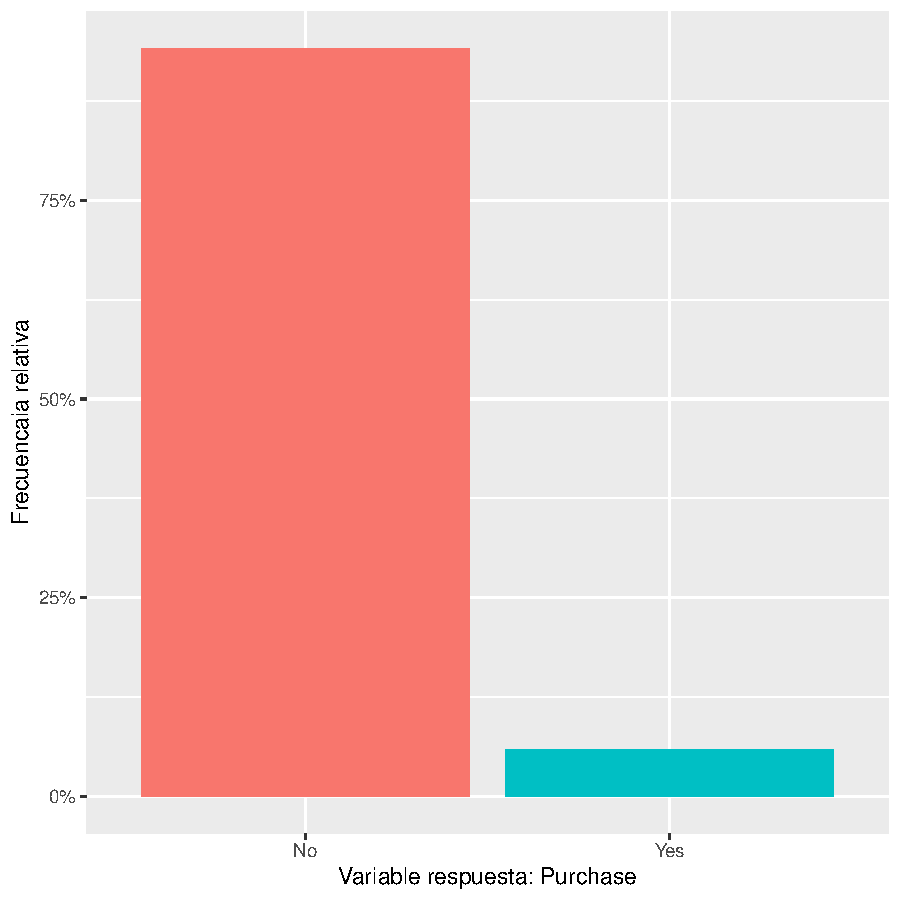
\includegraphics[width=.6\linewidth]{figure/NUEVAS1-SOLUCION-Rnwauto-report-1} 

}


\begin{kframe}\begin{alltt}
\hlcom{# Equilibramos las clases}
\hlstd{train.yes}\hlkwb{=}\hlstd{car.train[car.train}\hlopt{$}\hlstd{Purchase}\hlopt{==}\hlstr{"Yes"}\hlstd{,]}
\hlstd{size1}\hlkwb{=}\hlkwd{dim}\hlstd{(train.yes)[}\hlnum{1}\hlstd{]}
\hlstd{train.no}\hlkwb{=}\hlstd{car.train[car.train}\hlopt{$}\hlstd{Purchase}\hlopt{==}\hlstr{"No"}\hlstd{,]}
\hlstd{dimension2}\hlkwb{=}\hlkwd{dim}\hlstd{(train.no)[}\hlnum{1}\hlstd{]}
\hlstd{indices.no}\hlkwb{=}\hlkwd{sample}\hlstd{(}\hlnum{1}\hlopt{:}\hlstd{dimension2,}\hlkwc{size}\hlstd{=size1,}\hlkwc{replace}\hlstd{=}\hlnum{FALSE}\hlstd{)}
\hlstd{muestra.no}\hlkwb{=}\hlstd{train.no[indices.no,]}

\hlstd{car.train}\hlkwb{=}\hlkwd{rbind}\hlstd{(car.train[car.train}\hlopt{$}\hlstd{Purchase}\hlopt{==}\hlstr{"Yes"}\hlstd{,],muestra.no)}
\hlkwd{ggplot}\hlstd{(}\hlkwc{data}\hlstd{=car.train,}\hlkwd{aes}\hlstd{(}\hlkwc{x}\hlstd{=Purchase,}\hlkwc{fill}\hlstd{=Purchase))} \hlopt{+}
  \hlkwd{geom_bar}\hlstd{(}\hlkwd{aes}\hlstd{(}\hlkwc{y}\hlstd{=(..count..)}\hlopt{/}\hlkwd{sum}\hlstd{(..count..)))} \hlopt{+}
  \hlkwd{scale_y_continuous}\hlstd{(}\hlkwc{labels}\hlstd{=scales}\hlopt{::}\hlstd{percent)} \hlopt{+}
  \hlkwd{theme}\hlstd{(}\hlkwc{legend.position}\hlstd{=}\hlstr{"none"}\hlstd{)} \hlopt{+}
  \hlkwd{ylab}\hlstd{(}\hlstr{"Frecuencaia relativa"}\hlstd{)} \hlopt{+}
  \hlkwd{xlab}\hlstd{(}\hlstr{"Variable respuesta: Purchase"}\hlstd{)}
\end{alltt}
\end{kframe}

{\centering 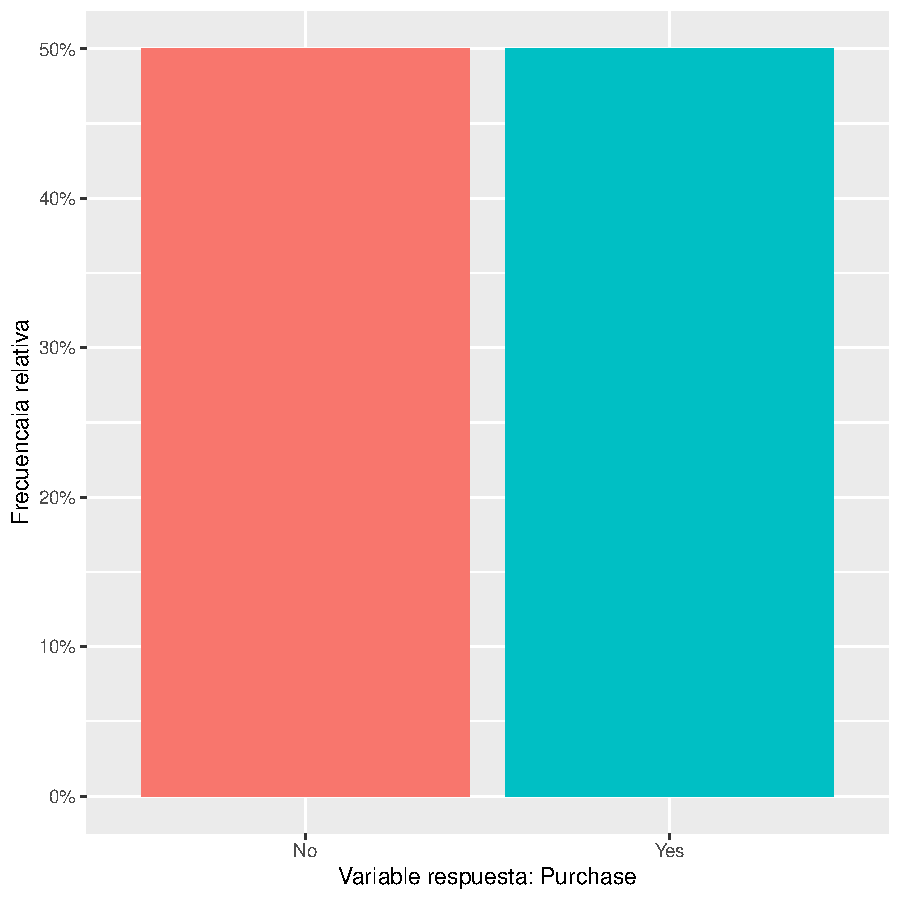
\includegraphics[width=.6\linewidth]{figure/NUEVAS1-SOLUCION-Rnwauto-report-2} 

}


\begin{kframe}\begin{alltt}
\hlcom{# Podemos comprobar como ahora la muestra de train está equilibrada}

\hlcom{# Ajustamos un modelo de random forest}
\hlkwd{library}\hlstd{(randomForest)}
\hlstd{rf} \hlkwb{<-}\hlkwd{randomForest}\hlstd{(Purchase}\hlopt{~}\hlstd{.,}\hlkwc{data}\hlstd{=car.train,} \hlkwc{ntree}\hlstd{=}\hlnum{300}\hlstd{)}
\hlkwd{print}\hlstd{(rf)}
\end{alltt}
\begin{verbatim}
## 
## Call:
##  randomForest(formula = Purchase ~ ., data = car.train, ntree = 300) 
##                Type of random forest: classification
##                      Number of trees: 300
## No. of variables tried at each split: 9
## 
##         OOB estimate of  error rate: 34.24%
## Confusion matrix:
##      No Yes class.error
## No  183  93   0.3369565
## Yes  96 180   0.3478261
\end{verbatim}
\begin{alltt}
\hlcom{# Importancia de las variables}
\hlkwd{importance}\hlstd{(rf)}
\end{alltt}
\begin{verbatim}
##          MeanDecreaseGini
## MOSTYPE       10.05904963
## MAANTHUI       0.97148706
## MGEMOMV        2.99982901
## MGEMLEEF       2.73945263
## MOSHOOFD       7.40132377
## MGODRK         3.11540474
## MGODPR         5.16206064
## MGODOV         3.54183796
## MGODGE         4.50020156
## MRELGE         6.29591228
## MRELSA         3.42708164
## MRELOV         4.57335346
## MFALLEEN       4.85879716
## MFGEKIND       4.78080394
## MFWEKIND       5.36700709
## MOPLHOOG       4.48465020
## MOPLMIDD       4.94601049
## MOPLLAAG       5.34765518
## MBERHOOG       4.64327851
## MBERZELF       2.29936647
## MBERBOER       1.99476918
## MBERMIDD       5.03094781
## MBERARBG       6.06600522
## MBERARBO       5.00942241
## MSKA           4.96233239
## MSKB1          4.43889944
## MSKB2          4.87845474
## MSKC           5.34422043
## MSKD           3.49028301
## MHHUUR         6.96107866
## MHKOOP         6.59897367
## MAUT1          6.00579172
## MAUT2          4.54617054
## MAUT0          4.49778685
## MZFONDS        4.77888012
## MZPART         4.54065956
## MINKM30        6.18548906
## MINK3045       5.10631946
## MINK4575       5.99601714
## MINK7512       3.11406923
## MINK123M       2.40521110
## MINKGEM        4.76788814
## MKOOPKLA       6.27471357
## PWAPART        3.25969479
## PWABEDR        0.37903843
## PWALAND        0.38711742
## PPERSAUT      18.85519843
## PBESAUT        0.13948725
## PMOTSCO        0.63245819
## PVRAAUT        0.00000000
## PAANHANG       0.36411184
## PTRACTOR       0.34404056
## PWERKT         0.05130278
## PBROM          0.68501334
## PLEVEN         1.39712238
## PPERSONG       0.08259973
## PGEZONG        0.17193584
## PWAOREG        0.45610190
## PBRAND         8.16546475
## PZEILPL        0.04105962
## PPLEZIER       1.03885525
## PFIETS         0.59262307
## PINBOED        0.10883277
## PBYSTAND       0.64658945
## AWAPART        2.82835739
## AWABEDR        0.23497898
## AWALAND        0.41269745
## APERSAUT      12.19875224
## ABESAUT        0.13026212
## AMOTSCO        0.53350872
## AVRAAUT        0.00000000
## AAANHANG       0.49234946
## ATRACTOR       0.45963421
## AWERKT         0.04249799
## ABROM          0.74700286
## ALEVEN         1.65339999
## APERSONG       0.11538694
## AGEZONG        0.13805431
## AWAOREG        0.38868734
## ABRAND         2.40158370
## AZEILPL        0.04393799
## APLEZIER       1.15358862
## AFIETS         0.68422159
## AINBOED        0.11516453
## ABYSTAND       0.63127388
\end{verbatim}
\begin{alltt}
\hlkwd{varImpPlot}\hlstd{(rf)}
\end{alltt}
\end{kframe}

{\centering 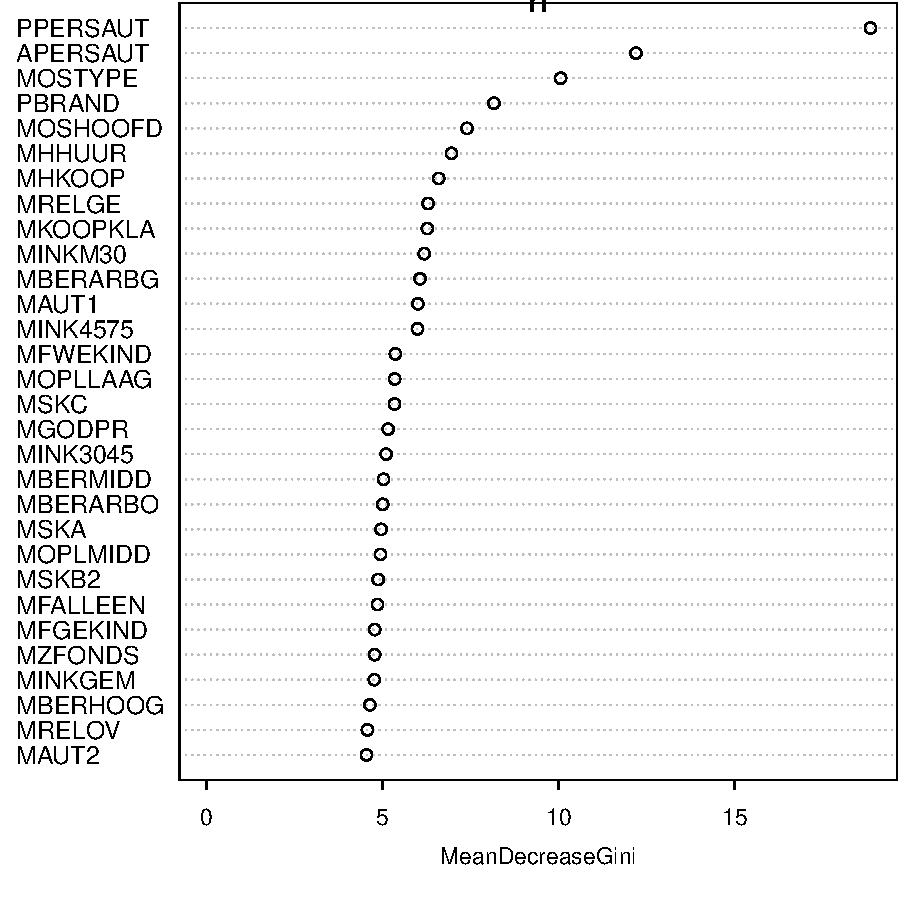
\includegraphics[width=.6\linewidth]{figure/NUEVAS1-SOLUCION-Rnwauto-report-3} 

}


\begin{kframe}\begin{alltt}
\hlcom{# Curva ROC}
\hlstd{pred1}\hlkwb{=}\hlkwd{predict}\hlstd{(rf,car.test,}\hlkwc{type} \hlstd{=} \hlstr{"prob"}\hlstd{)}
\hlstd{perf} \hlkwb{=} \hlkwd{prediction}\hlstd{(pred1[,}\hlnum{2}\hlstd{], car.test}\hlopt{$}\hlstd{Purchase)}
\hlcom{# True Positive y Negative Rate}
\hlstd{pred3} \hlkwb{=} \hlkwd{performance}\hlstd{(perf,} \hlstr{"tpr"}\hlstd{,}\hlstr{"fpr"}\hlstd{)}
\hlcom{# ROC }
\hlkwd{plot}\hlstd{(pred3,}\hlkwc{main}\hlstd{=}\hlstr{"Curva ROC para el Random Forest"}\hlstd{,}\hlkwc{col}\hlstd{=}\hlnum{2}\hlstd{,}\hlkwc{lwd}\hlstd{=}\hlnum{2}\hlstd{,}
     \hlkwc{xlab}\hlstd{=}\hlstr{"Tasa de falsos positivos"}\hlstd{,}\hlkwc{ylab}\hlstd{=}\hlstr{"Tasa de verdaderos positivos"}\hlstd{)}
\hlkwd{abline}\hlstd{(}\hlkwc{a}\hlstd{=}\hlnum{0}\hlstd{,}\hlkwc{b}\hlstd{=}\hlnum{1}\hlstd{,}\hlkwc{lwd}\hlstd{=}\hlnum{2}\hlstd{,}\hlkwc{lty}\hlstd{=}\hlnum{2}\hlstd{,}\hlkwc{col}\hlstd{=}\hlstr{"gray"}\hlstd{)}
\end{alltt}
\end{kframe}

{\centering 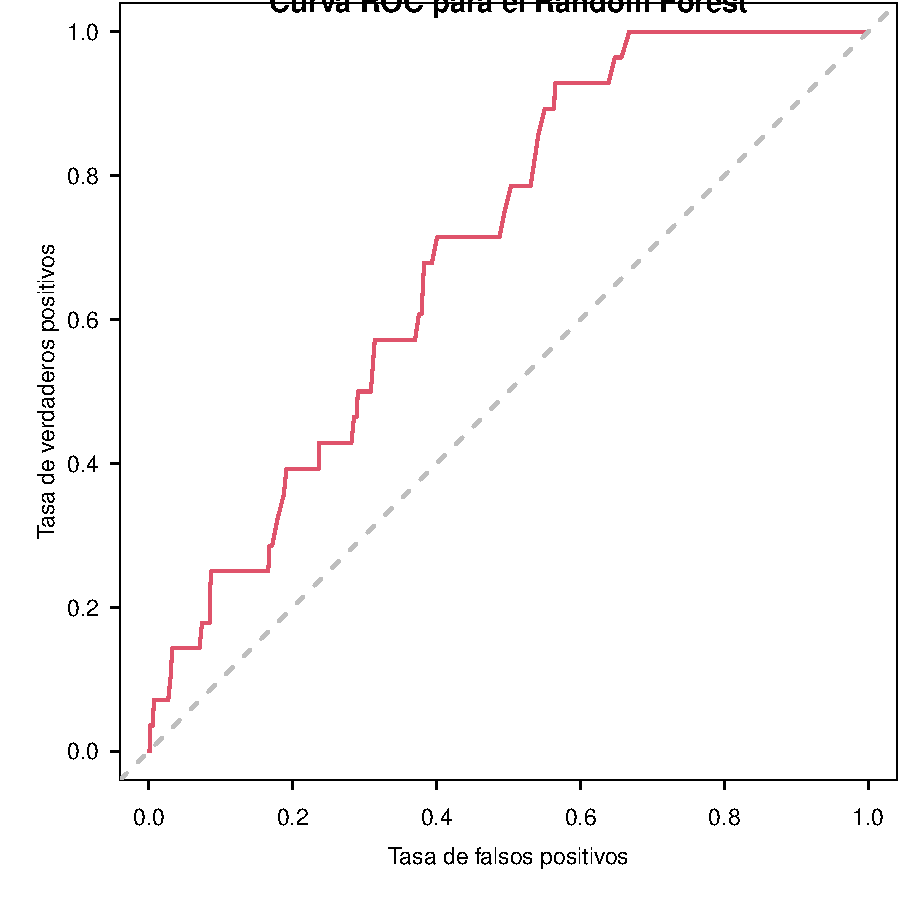
\includegraphics[width=.6\linewidth]{figure/NUEVAS1-SOLUCION-Rnwauto-report-4} 

}


\begin{kframe}\begin{alltt}
\hlstd{explain_rf} \hlkwb{<-} \hlstd{DALEX}\hlopt{::}\hlkwd{explain}\hlstd{(}\hlkwc{model} \hlstd{= rf,}
                             \hlkwc{data} \hlstd{= car.test,}
                             \hlkwc{y} \hlstd{= car.test}\hlopt{$}\hlstd{Purchase,}
                             \hlkwc{label} \hlstd{=} \hlstr{"Random Forest"}\hlstd{)}
\end{alltt}
\begin{verbatim}
## Preparation of a new explainer is initiated
##   -> model label       :  Random Forest 
##   -> data              :  582  rows  86  cols 
##   -> target variable   :  582  values 
##   -> predict function  :  yhat.randomForest  will be used (  default  )
##   -> predicted values  :  No value for predict function target column. (  default  )
##   -> model_info        :  package randomForest , ver. 4.7.1.1 , task classification (  default  ) 
##   -> model_info        :  Model info detected classification task but 'y' is a factor .  (  WARNING  )
##   -> model_info        :  By deafult classification tasks supports only numercical 'y' parameter. 
##   -> model_info        :  Consider changing to numerical vector with 0 and 1 values.
##   -> model_info        :  Otherwise I will not be able to calculate residuals or loss function.
##   -> predicted values  :  numerical, min =  0.01333333 , mean =  0.4199771 , max =  0.95  
##   -> residual function :  difference between y and yhat (  default  )
\end{verbatim}


{\ttfamily\noindent\color{warningcolor}{\#\# Warning in Ops.factor(y, predict\_function(model, data)): '-' not meaningful for factors}}\begin{verbatim}
##   -> residuals         :  numerical, min =  NA , mean =  NA , max =  NA  
##   A new explainer has been created!
\end{verbatim}
\begin{alltt}
\hlstd{obs1}\hlkwb{=}\hlstd{car.test[}\hlnum{1}\hlstd{,]}
\hlstd{obs2}\hlkwb{=}\hlstd{car.test[}\hlnum{2}\hlstd{,]}

\hlkwd{predict}\hlstd{(explain_rf, obs1)}
\end{alltt}
\begin{verbatim}
## [1] 0.1933333
\end{verbatim}
\begin{alltt}
\hlkwd{predict}\hlstd{(explain_rf, obs2)}
\end{alltt}
\begin{verbatim}
## [1] 0.32
\end{verbatim}
\begin{alltt}
\hlstd{shap_obs1} \hlkwb{<-} \hlkwd{predict_parts}\hlstd{(}\hlkwc{explainer} \hlstd{= explain_rf,}
                            \hlkwc{new_observation} \hlstd{= obs1,}
                            \hlkwc{type} \hlstd{=} \hlstr{"shap"}\hlstd{,}
                            \hlkwc{B} \hlstd{=} \hlnum{25}\hlstd{)}

\hlkwd{plot}\hlstd{(shap_obs1,} \hlkwc{show_boxplots} \hlstd{=} \hlnum{FALSE}\hlstd{)}
\end{alltt}
\end{kframe}

{\centering 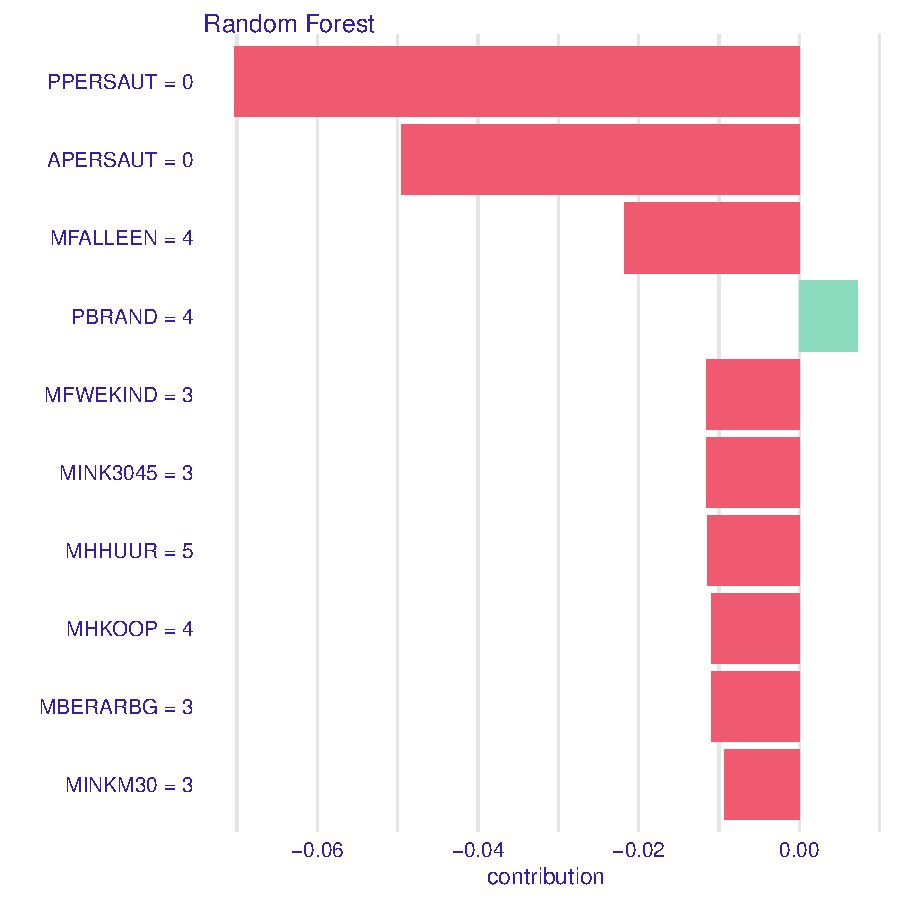
\includegraphics[width=.6\linewidth]{figure/NUEVAS1-SOLUCION-Rnwauto-report-5} 

}


\begin{kframe}\begin{alltt}
\hlstd{shap_obs2} \hlkwb{<-} \hlkwd{predict_parts}\hlstd{(}\hlkwc{explainer} \hlstd{= explain_rf,}
                            \hlkwc{new_observation} \hlstd{= obs2,}
                            \hlkwc{type} \hlstd{=} \hlstr{"shap"}\hlstd{,}
                            \hlkwc{B} \hlstd{=} \hlnum{25}\hlstd{)}
\hlkwd{plot}\hlstd{(shap_obs2,} \hlkwc{show_boxplots} \hlstd{=} \hlnum{FALSE}\hlstd{)}
\end{alltt}
\end{kframe}

{\centering 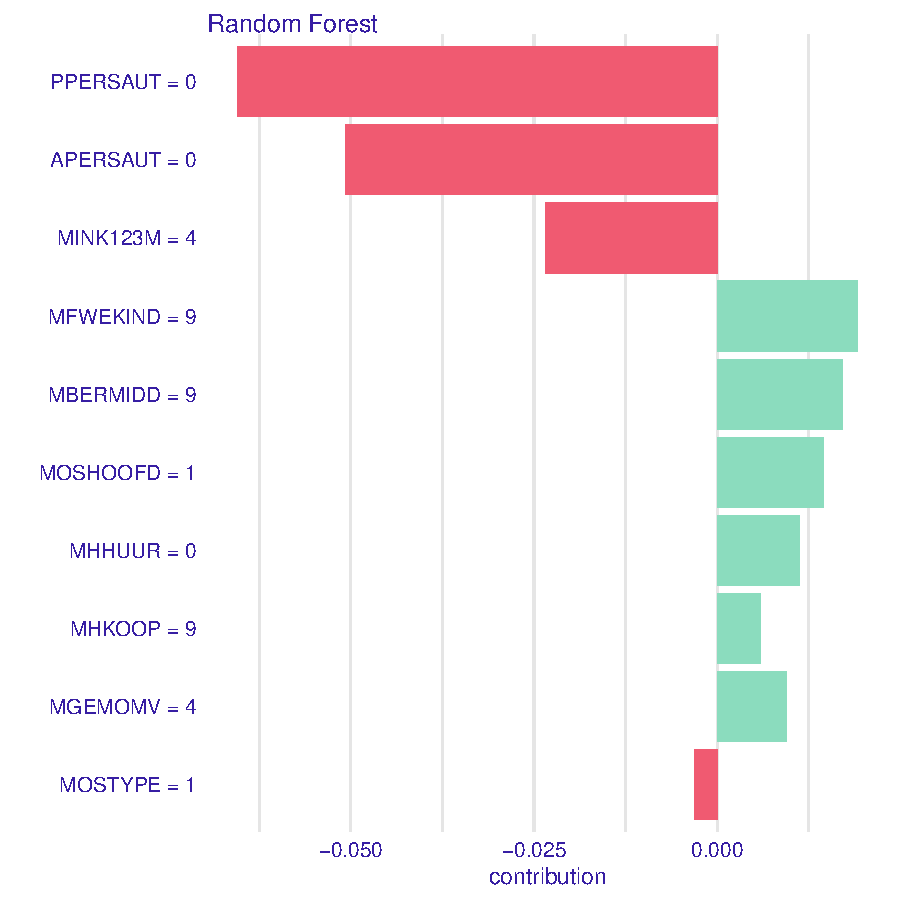
\includegraphics[width=.6\linewidth]{figure/NUEVAS1-SOLUCION-Rnwauto-report-6} 

}


\end{knitrout}

The R session information (including the OS info, R version and all
packages used):

\begin{knitrout}
\definecolor{shadecolor}{rgb}{0.969, 0.969, 0.969}\color{fgcolor}\begin{kframe}
\begin{alltt}
\hlkwd{sessionInfo}\hlstd{()}
\end{alltt}
\begin{verbatim}
## R version 4.3.1 (2023-06-16)
## Platform: x86_64-pc-linux-gnu (64-bit)
## Running under: Ubuntu 20.04.6 LTS
## 
## Matrix products: default
## BLAS:   /usr/lib/x86_64-linux-gnu/atlas/libblas.so.3.10.3 
## LAPACK: /usr/lib/x86_64-linux-gnu/atlas/liblapack.so.3.10.3;  LAPACK version 3.9.0
## 
## locale:
##  [1] LC_CTYPE=es_ES.UTF-8       LC_NUMERIC=C               LC_TIME=es_ES.UTF-8       
##  [4] LC_COLLATE=es_ES.UTF-8     LC_MONETARY=es_ES.UTF-8    LC_MESSAGES=es_ES.UTF-8   
##  [7] LC_PAPER=es_ES.UTF-8       LC_NAME=C                  LC_ADDRESS=C              
## [10] LC_TELEPHONE=C             LC_MEASUREMENT=es_ES.UTF-8 LC_IDENTIFICATION=C       
## 
## time zone: Europe/Madrid
## tzcode source: system (glibc)
## 
## attached base packages:
## [1] stats     graphics  grDevices utils     datasets  methods   base     
## 
## other attached packages:
##  [1] DALEX_2.4.3          ROCR_1.0-11          randomForest_4.7-1.1 arulesViz_1.5-2     
##  [5] arules_1.7-6         Matrix_1.6-1.1       liver_1.15           ggfortify_0.4.16    
##  [9] factoextra_1.0.7     mlbench_2.1-3.1      readxl_1.4.3         caret_6.0-94        
## [13] lattice_0.21-9       ggplot2_3.4.3        rpart.plot_3.1.1     rpart_4.1.19        
## [17] caTools_1.18.2       dplyr_1.1.3          ISLR2_1.3-2         
## 
## loaded via a namespace (and not attached):
##  [1] bitops_1.0-7         pROC_1.18.4          gridExtra_2.3        rlang_1.1.1         
##  [5] magrittr_2.0.3       e1071_1.7-13         compiler_4.3.1       vctrs_0.6.3         
##  [9] reshape2_1.4.4       stringr_1.5.0        crayon_1.5.2         pkgconfig_2.0.3     
## [13] fastmap_1.1.1        ellipsis_0.3.2       labeling_0.4.3       ggraph_2.1.0        
## [17] utf8_1.2.3           rmarkdown_2.25       prodlim_2023.08.28   tzdb_0.4.0          
## [21] tinytex_0.47         purrr_1.0.2          xfun_0.40            jsonlite_1.8.7      
## [25] recipes_1.0.8        highr_0.10           tweenr_2.0.2         parallel_4.3.1      
## [29] R6_2.5.1             stringi_1.7.12       parallelly_1.36.0    lubridate_1.9.3     
## [33] cellranger_1.1.0     Rcpp_1.0.11          iterators_1.0.14     knitr_1.44          
## [37] future.apply_1.11.0  readr_2.1.4          splines_4.3.1        nnet_7.3-19         
## [41] igraph_1.5.1         timechange_0.2.0     tidyselect_1.2.0     rstudioapi_0.15.0   
## [45] yaml_2.3.7           viridis_0.6.4        timeDate_4022.108    codetools_0.2-19    
## [49] listenv_0.9.0        tibble_3.2.1         plyr_1.8.9           withr_2.5.1         
## [53] evaluate_0.22        future_1.33.0        survival_3.5-7       proxy_0.4-27        
## [57] polyclip_1.10-6      pillar_1.9.0         foreach_1.5.2        stats4_4.3.1        
## [61] generics_0.1.3       hms_1.1.3            munsell_0.5.0        scales_1.2.1        
## [65] globals_0.16.2       class_7.3-22         glue_1.6.2           tools_4.3.1         
## [69] data.table_1.14.8    ModelMetrics_1.2.2.2 gower_1.0.1          visNetwork_2.1.2    
## [73] graphlayouts_1.0.1   tidygraph_1.2.3      grid_4.3.1           tidyr_1.3.0         
## [77] iBreakDown_2.0.1     ipred_0.9-14         colorspace_2.1-0     nlme_3.1-163        
## [81] ggforce_0.4.1        cli_3.6.1            fansi_1.0.5          viridisLite_0.4.2   
## [85] lava_1.7.2.1         gtable_0.3.4         digest_0.6.33        ggrepel_0.9.3       
## [89] htmlwidgets_1.6.2    farver_2.1.1         htmltools_0.5.6.1    lifecycle_1.0.3     
## [93] hardhat_1.3.0        MASS_7.3-60
\end{verbatim}
\begin{alltt}
\hlkwd{Sys.time}\hlstd{()}
\end{alltt}
\begin{verbatim}
## [1] "2023-11-02 20:21:22 CET"
\end{verbatim}
\end{kframe}
\end{knitrout}


\end{document}
